\begin{figure}
    \begin{fullwidth}
    \centering
    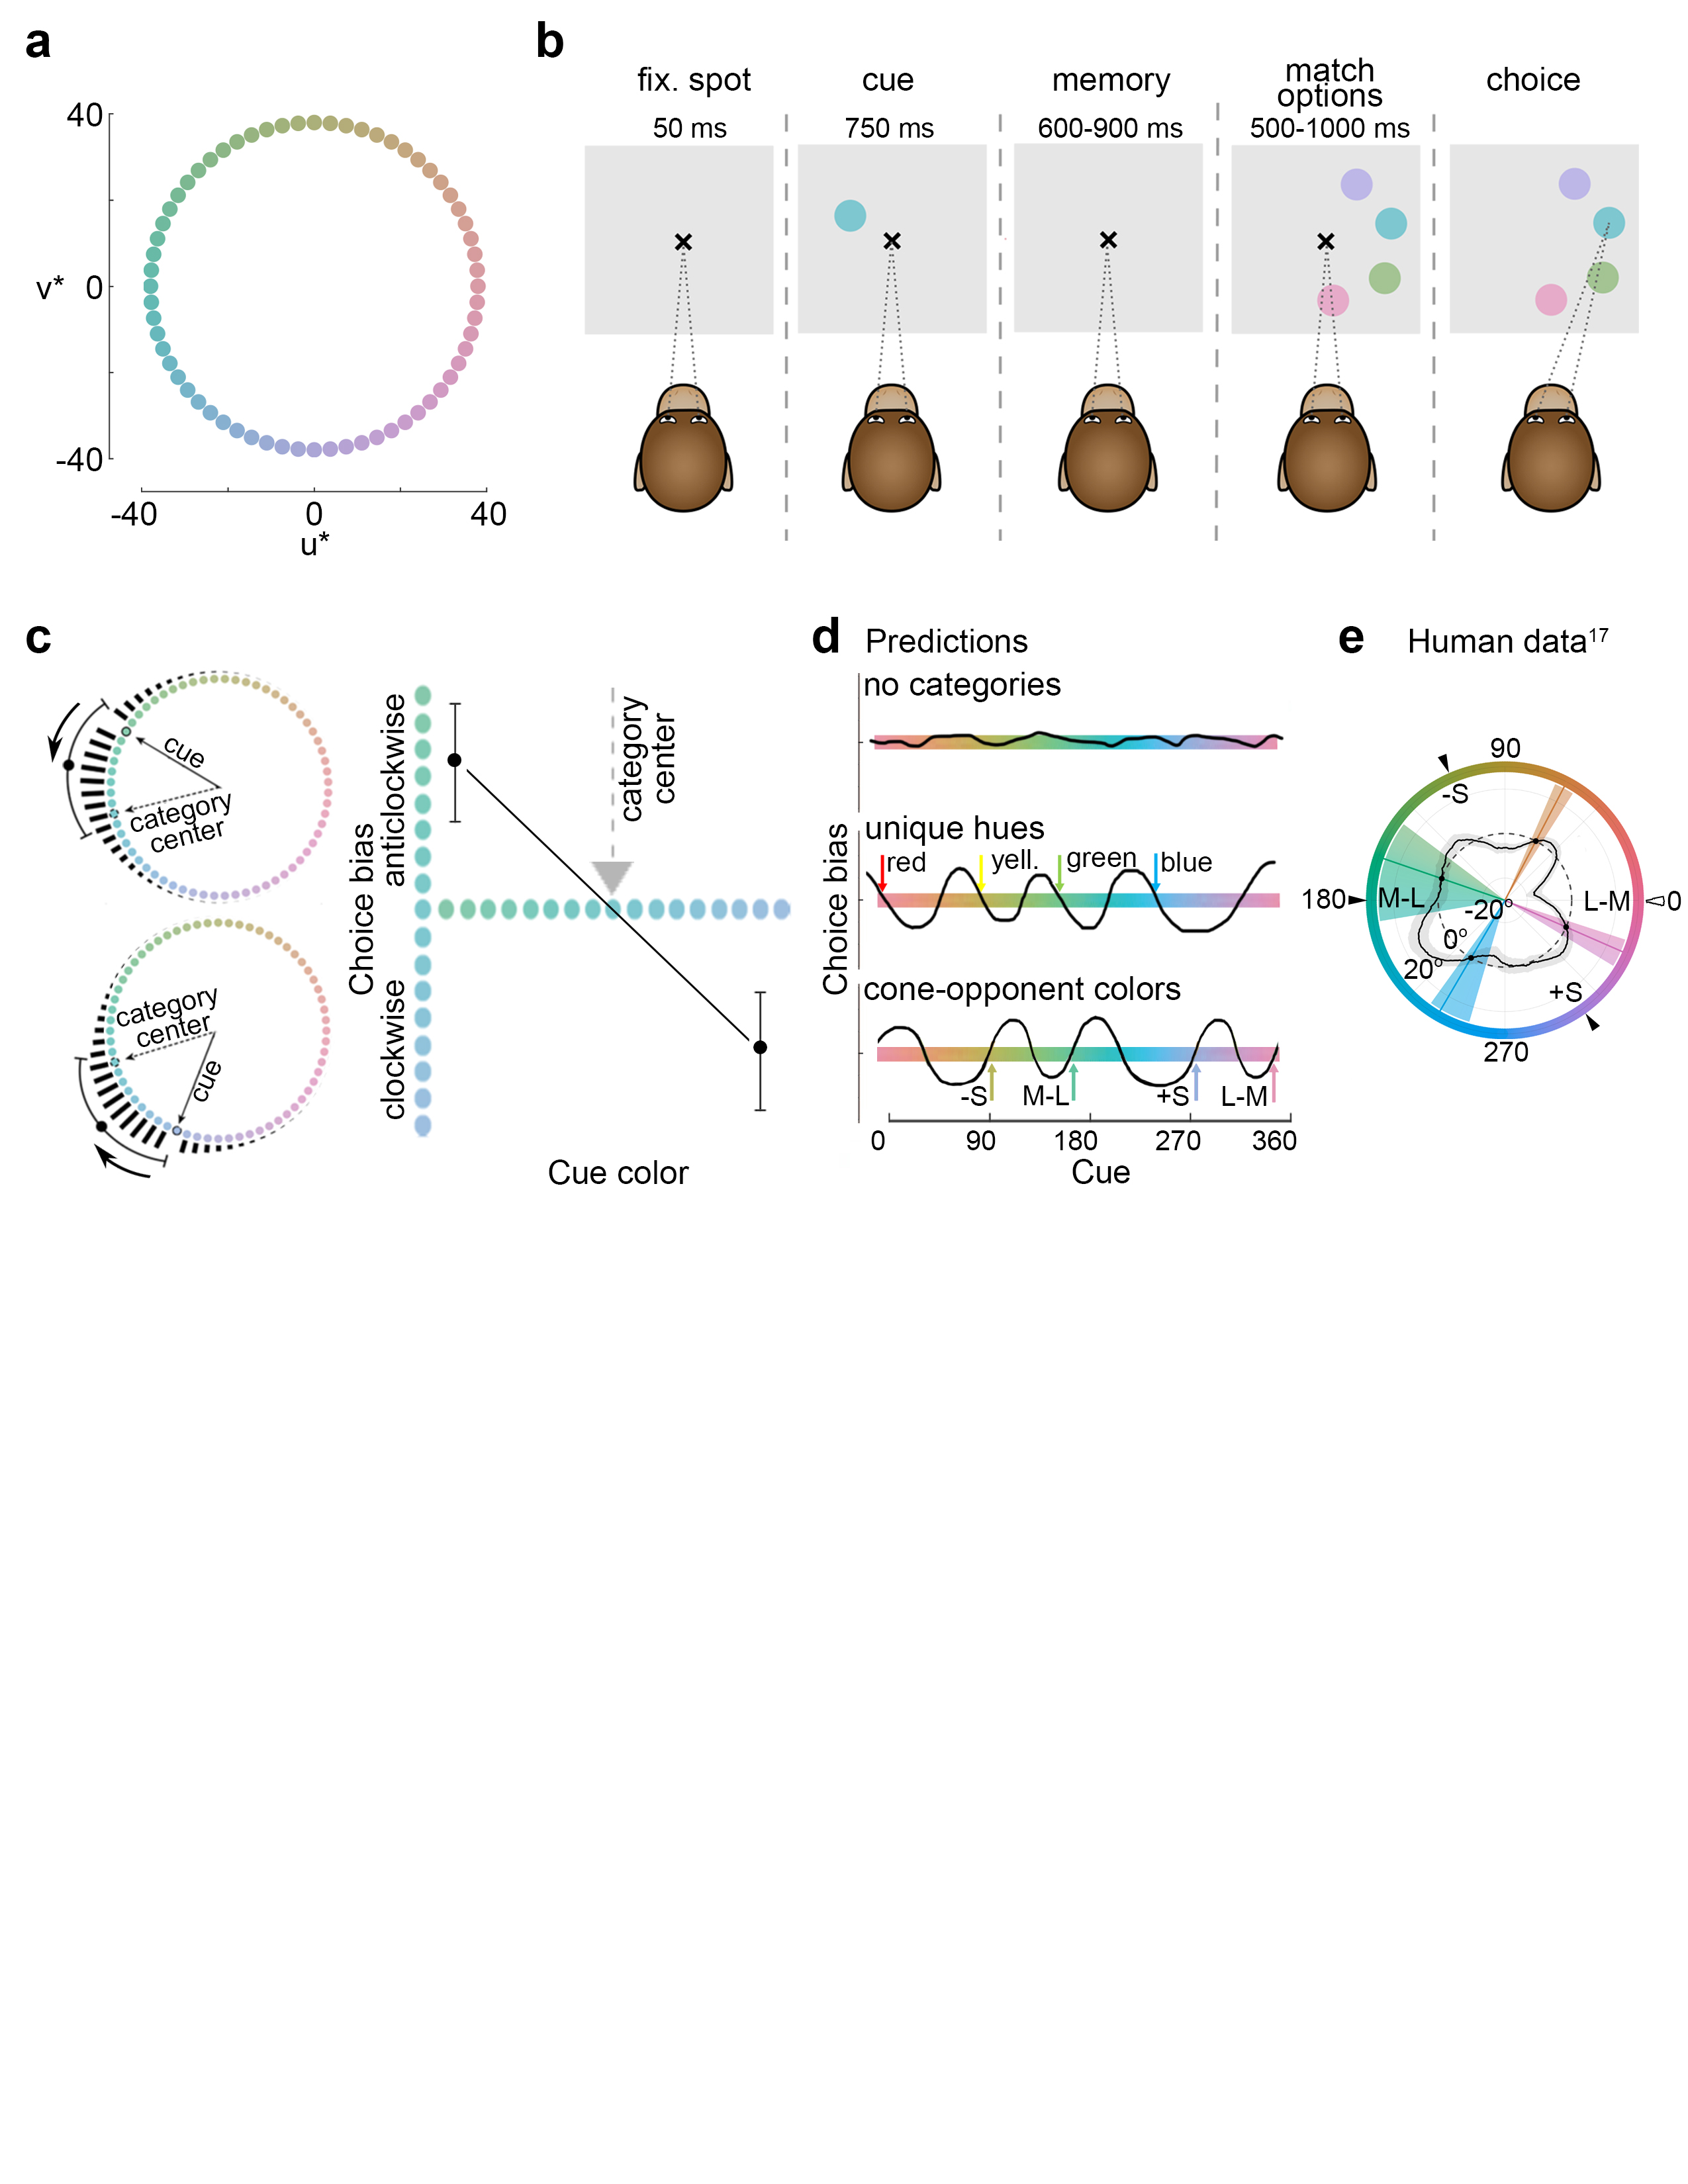
\includegraphics[width=\textwidth+4cm,trim={0 12.5cm 0 0},clip]{../Figures/flat/F1_ParadigmPredictions_8.jpg}
    \caption{\textbf{Non-verbal paradigm to recover color categories in non-human primates.}
    \textbf{a}, Sixty-four Colors defined in CIELUV color space. 
	\textbf{b}, Animals were trained to initiate a trial by fixating a small cross on a computer monitor and to maintain fixation throughout the trial until the fixation cross disappeared, which was their instruction to make a choice; trials in which the animals broke fixation were aborted. 
	A 3-degree diameter cue was presented within the central 2.5 – 6-degrees, followed by a variable memory delay (600-900ms) and the presentation of four choice options. 
	To mitigate impulsive choices, the choice options were shown for a variable amount of time (500-1000 ms) during which the animals needed to maintain fixation to avoid aborting the trial. After the fixation cross disappeared, the animals were free to make their selection. 
	\textbf{c}, Predicted distribution of choices for two cues if a color category exists at the specified location in the color space (dashed arrow). 
	The average of the distribution of choices will be biased counterclockwise from the cue if the cue is displaced clockwise to the category center (top) and biased clockwise from the cue if the cue is displaced counterclockwise to the category center (bottom). This pattern of results would be captured as the zero-crossing of the negative slope in a plot of the choice bias versus cue color (right). 
	\textbf{d}, Predicted pattern of results for three hypotheses: no categories (top); categories defined by attractors to the four common basic color categories (middle); and categories defined by repellors to the cone-opponent retinal encoding mechanisms (bottom). 
	\textbf{e}, Data obtained in prior work on a related task in human subjects showing evidence of four color categories. Data shown are from \citet{panichello_error-correcting_2019}; see SI Figure 2 for three other data sets in human subjects including the original work from \citet{bae_why_2015} and new data using the present task, all infer the existence of four consensus color categories. The negative slopes demarking category centers are recovered by tracing the line in a counterclockwise direction, at points where the trace crosses the dashed circle marking zero choice bias. For reference, arrowheads show the colors that would isolate the retinal cone-opponent encoding mechanisms (L-M, M-L, +S, -S; where L, M, S are the three cone types).}
    \label{fig:ParadigmAnalysisPredictions}
    \end{fullwidth}
\end{figure}

Color categories are identified by color terms, of which the Basic Color Terms are considered prominent \citep{berlin_basic_1969}.
One hypothesis is that a subset of these terms---red, green, blue, yellow---express universal concepts \citep{heider_universals_1972,regier_focal_2005}
that are endowed by hard-wired neural mechanisms present at birth \citep{bornstein_categories_1976,lindsey_universality_2006}. 
This idea, put forth 150 years ago \citep{hering_zur_1875}, predicts common patterns in color naming across cultures \citep{baronchelli_modeling_2010,lindsey_hunter-gatherer_2015,abbott_focal_2016}
and finds some neurophysiological support in human infants \citep{clifford_electrophysiological_2009,yang_cortical_2016}. 
Behavioral work in infants also provides evidence for a biological origin of color categories \citep{franklin_new_2004,ozturk_language_2013} and suggests that color categories may build on an innate scaffolding defined by retinal cone-opponent mechanisms \citep{skelton_biological_2017}. The infants in all these experiments were at least several months old, by which stage they would have had substantial cultural exposure, so the evidence that they express color categories cannot be conclusively ascribed to an innate origin. Another hypothesis is that color categories emerge in development, instructed by language and culture \citep{davidoff_colour_1999,roberson_color_2005}, possibly involving an interplay of innate and developmental factors \citep{webster_variations_2002,kay_language_2006,franklin_lateralization_2008,regier_language_2009,paramei_online_2018}. Support for this hypothesis is provided by the variability in color-naming patterns across languages \citep{davidoff_colour_1999,webster_variations_2002,roberson_color_2005,kay_language_2006,gibson_color_2017, paramei_online_2018}. Current consensus is that at least some aspect of color category behavior is acquired through experience. But the extent to which color categories are innate remains unresolved \citep{davidoff_nature_2009,RN18696,RN18699}(see also chapter 6 in \citep{block_border_2023}).

Another approach to studying the origin of color categories could be provided by behavioral experiments in trichromatic non-human primates \citep{sandell_color_1979,carey_where_2009,RN18699,siuda-krzywicka_biological_2019} since they lack language but have almost identical perceptual systems to humans and presumably the same perceptual color space \citep{schnapf_spectral_1987,stoughton_psychophysical_2012,gagin_color-detection_2014, horwitz_what_2015}. The few studies on this topic have come to different conclusions: one found color categories in macaque monkeys consistent with categories in human adults \citep{sandell_color_1979}, implying that color categories do not depend on language and may be innate.
This study inadvertently made comparisons substantially easier for cross-category than within-category trials, undermining its conclusion \citep{davidoff_cross-species_2010}. 
A later study tested for the existence of color categories across a limited range of colors and found a blue-green boundary in humans but not baboons \citep{fagot_cross-species_2006,RN18699}. The lack of color categories in the baboons might reflect the limited survey of color space (blues and greens are categorized with high variability in all languages, including English \citep{gibson_color_2017}). A third study, designed to investigate visual working memory, uncovered a different pattern of results in the two animals tested \citep{panichello_error-correcting_2019}, raising the possibility that the two animals had private color categories. 

\paragraph{Measuring color categories in macaque monkeys}

Addressing the question of color categories in monkeys requires overcoming several challenges. First, how can color categories be measured non-verbally, without teaching the animals the categories or reinforcing idiosyncratic biases \citep{essock_color_1977,matsuno_color_2004}? Second, how should the color stimuli be specified \citep{siuda-krzywicka_biological_2019}? For example, specifying the colors as wavelengths \citep{sandell_color_1979} is not appropriate \citep{davidoff_cross-species_2010}. 
Third, how can data across the full circle of hues be obtained so as to avoid missing categories \citep{fagot_cross-species_2006}? A match-to-sample paradigm, using colors defined in a perceptually uniform color space \citep{stockman_colorimetry_2010} (Figure 1a), provides a potential solution to these challenges, because, as demonstrated for human subjects, color categories introduce biases in the distribution of matches \citep{bae_why_2015}. So color categories could be inferred from any observed biases across the space of colors without requiring participants to understand or produce linguistic labels.  

In the standard paradigm used in many experiments on working memory \citep{wilken_detection_2004,zhang_discrete_2008,panichello_error-correcting_2019,schurgin_psychophysical_2020} and adopted by \citet{bae_why_2015} to infer color categories, the subject is asked to match the color of a cue to a continuous ring of colors. This works in human participants who can follow instructions but introduces complications in monkeys because it is not clear how to reward the animals. Rewarding them for picking a color in the vicinity of the color of the cue could reinforce idiosyncratic biases, which is not a problem for addressing certain questions \citep{panichello_error-correcting_2019} but would be a problem for recovering consensus categories; moreover, the response metric (an eye movement or pointed finger) could confound the perceptual decision with motor noise. To overcome these complications, we adapted the paradigm as an alternative-forced-choice task in which a direct match to the cue was available in every trial and the monkeys were only rewarded for making the direct match with an eye movement (Figure 1b). The precision of the eye tracker (\textasciitilde0.3 degrees of visual angle) was considerably finer than the size of the choice options (3 degree diameter). One consequence of the adapted paradigm is that it requires a much larger number of trials to satisfactorily assess the similarity relationships of each color to every other color. Four animals performed the task, completing a total of 209456 trials over 232 sessions (SI Figure 1).

If a monkey has a color category, the category center will be an attractor in the color space. An attractor would be captured by a zero-crossing of negative slope in a plot of choice bias (Figure 1c). Repellors, meanwhile, would be captured by zero-crossings of positive slope. The approach is data-driven, so it will recover whatever categories exist; nonetheless, before collecting the data we considered three possibilities. First, that the monkeys would show no color categories, predicted by the work sampling a limited range of colors in baboons \citep{davidoff_cross-species_2010} (Figure 1d, top). Second, that the monkeys would show four color categories, predicted by attractor points defined by the four putatively universal basic color terms (Figure 1d, middle). Third, that the monkeys would show four color categories, but predicted by data in human infants corresponding to repellor points defined by physiological cone-opponent mechanisms not basic color terms \citep{skelton_biological_2017} (Figure 1d, bottom). For reference, Figure 1e shows the results in human adults \citep{panichello_error-correcting_2019}. These results have been replicated in English speakers by several groups, across multiple versions of the task, including by us, using the discrete-matching version used presently (SI Figure 2). The data recovers four color categories, although they do not perfectly line up with the four common basic terms. Instead they correspond to pink, orange, green, blue. The discrepancy may arise because of limitations imposed by ensuring equal saturation and luminance among the colors (the resulting set of stimuli has neither a good red nor a good yellow) (see \citep{bae_why_2015}). 
